\section{Applications} \label{section:applications}
The structured scene representation facilitates novel applications.  In
this paper, we demonstrate the following four.
Please also see our supplementary video.

\mysubsubsection{Floorplan generation}
%Given the precise shape and segmentation of architectural components,
The first application is the generation of floorplan images. One missing
information is the types of objects and rooms, which are obtained by
state-of-the-art object recognition
software~\cite{berkeley_object_detection_software} and scene recognition
software~\cite{mit_scene_demo_paper}.
%Simply throwing the panorama images did not work well, in particular for
%the scene recognition, and we have experimented several different
%algorithms to generate input images.
% Due to the space limitation,
Experimental details and evaluations are in the supplementary material.
% We restrict our description to the most interesting finding here, while
% referring the rest to the supplementary material. The scene recognition
% did not work well with the panorama images, and we render $400\times
% 300$ standard perspective images with the horizontal field of view of
% $90$ degrees. The results depend on the viewing directions and we
% experimented with the four algorithms as shown in
% Table~\ref{table:scene}.  The first algorithm, for example, picks the
% panorama closest to the room center, renders six uniformly overlapping
% images, and picks the scene type with the best average score. This
% performs the worst. The best algorithm looks at all the panorama images
% that are inside the room, but uses the single rendered image in which
% the room is the most visible in the top-down view. An observation is
% that poorly positioned panoramas tend to yield incorrect results but
% with very high confidence. A rather better strategy is to use the best
% viewing direction from the best panorama.
In addition to placing annotation texts,
%on the floorplan image,
we can automatically change the rendering style of each room and object
depending on its type.
%(\eg, background color and texture) and/or each object (\eg, icon
%choices).
%Please see our supplementary video for examples.

\mysubsubsection{Indoor scene viewer} Our model enables a
novel indoor scene viewer, which renders an indoor scene from ground to
air, shows the floorplan image, displays room thumbnails,
or highlights room structures.
%or visualizes the relationships among different structural elements.
Room elements serve as interactive icons to enable a room-based
navigation.

\mysubsubsection{Inverse-CAD} The mesh model compiled from the structure
graph is compact, yet regularized, and a manifold. We can export our
model to a CAD system (\eg Sketchup~\cite{sketchup} as COLLADA format)
for users to easily fix mistakes, add new structures, or clone new rooms
within a minute or two.

\mysubsubsection{Tunable reconstruction} As mobile applications
dominate, it becomes crucial to intuitively and directly control the
complexity of a model, because the computational powers of mobile
devices vary but are limited.
%Existing methods typically offer only scalar weights inside an energy
%function to control model smoothness. They are far from intuitive and
%often not effectivein controlling the model complexity.
%provide almost no effective control over the model complexity,
The structure graph allows us to,
%intuitively control the complexity of an output model,
for example, specify the maximum number of poygons allowed for an entire
scene (X), each room (Y), and each wall (Z). These constraints can be
easily enforced by repeatedly dropping leaf nodes until satisfaction
%We simply repeat dropping leaf nodes until these constraints are all
%satisfied
(See Fig.~\ref{fig:complexity_control}).
\begin{figure}[!t]
\begin{center}
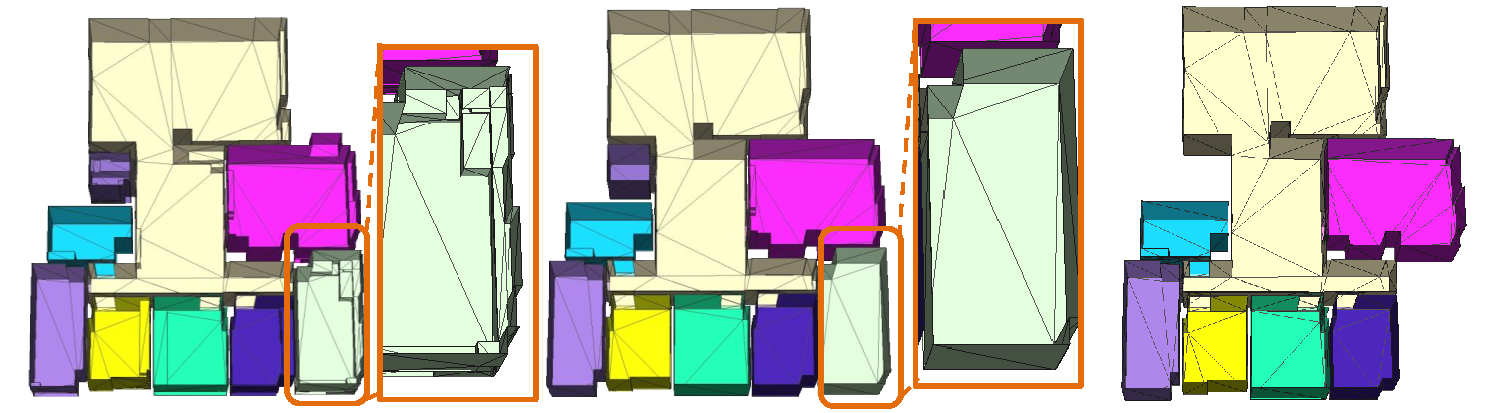
\includegraphics[width=85mm]{../figures/complexity2.pdf}
\end{center}
 \vspace{-0.2cm}
\caption{Structured model representation allows one to
 directly specify the
 % intuitively  control the complexity of an output manifold mesh, in particular, the
 maximum number of polygons allowed for an entire scene (X), each room
 (Y), and each wall (Z). The values of $(X,Y,Z)$ are $(2000,500,100)$,
 $(1000, 500, 2)$, and $(500, 100, 10)$ from left to right in the figure.
 When the budget is really tight (right), the
 system might drop a few rooms. %, yet the model is a manifold without gaps
 % or holes, and prevents artifacts in rendering and simulation.
 %
%  Mesh complexity control based on our graph structure. Using our
% model representation, we can easTily control the complexity of manifold
% meshes for each element-level. In this example, we fix the maximum
% number of meshes about (entire scene, each room, each wall) and then
% automatically compiled corresponding meshes. The mesh models at (left)
% is more complex than (middle), and some room geometry was dropped in
% (right) but the manifold-ness is still satisfied. \yasu{this will be
%  important for mobile application, where the rendering power varies
%  depending on the device but  is limited. The manifold mesh without gaps
%  and holes is ideal for rendering and simulation.
 }
\label{fig:complexity_control}
 \vspace{-0.25cm}
\end{figure}

% Note that most existing reconstruction algorithms usually provide a few
% mysterious parameters (\eg, scalar weights in the MRF formulation),
% where these parameters are non-intuitive, and resultant models are
% highly unpredictable.

%         %algorithm and exact parameters. Can you provide here?} We also
% %remove objects that are near walls, which can be represented by room
% mesh model \yasu{again how exactly?}. To do this, we discretize the 3D
% room space to $64\times 64\times 64$ voxels and mark voxels that are
% occupied by room structures as 1 and all others as 0. After dialating
% the voxel grid, we remove objects whose more than 75\% of points are
% inside voxels with value 1. The next step is to re-assign colors to
% objects points from panoramas since the original colors are not
% reliable. The key point here is to select a minimum set of panoramas
% from which the most points of the object can be clearly seen. Given an
% object, we initialize all points as unseen, and greedily search for
% panoramas in which the object occupies largest area in image domain, and
% most unseen points become seen. To compensate for exposure difference
% between panoramas, we also estimate a $3\times 3$ color transform matrix
% between two panoramas using the points that can be seen from both of
% them.
